\documentclass[10pt,twocolumn,letterpaper]{article}
\usepackage{times}
\usepackage{graphicx}
\usepackage{amsmath,amssymb}
\usepackage{booktabs}
\usepackage{multirow}
\usepackage{array}
\usepackage{url}
\usepackage{xcolor}
\usepackage{caption}
\usepackage{enumitem}
\usepackage{microtype}
\usepackage{hyperref}
\hypersetup{colorlinks=true,allcolors=blue!55!black}
\setlength{\textwidth}{6.875in}
\setlength{\textheight}{8.875in}
\setlength{\columnsep}{0.3125in}
\setlength{\topmargin}{0in}
\setlength{\headheight}{0in}
\setlength{\headsep}{0in}
\setlength{\oddsidemargin}{-0.1875in}
\setlength{\evensidemargin}{-0.1875in}
\setlength{\parindent}{1pc}
\setlength{\parskip}{0pt}
\captionsetup{font=small,labelfont=bf}
\setlist{nosep,leftmargin=*}
\newcommand{\pp}{\,\mathrm{pp}}
\newcommand{\samme}{\textsc{SAMME}}
\title{Decision Trees, Bagging, and Multiclass \samme{} on Olivetti Faces: Robustness and Measured Bias--Variance}
\author{Aarish Quazi\\Roll No. M26MER008\\Indian Institute of Technology Jodhpur\\\small GitHub: \url{https://github.com/aarishquazi/ML_ASSIGNMENT2}\\\small Final GitHub commit: \texttt{0f344a62a0bb94ea2987cf90b1543de24a17b052}}
\date{}
\begin{document}
\maketitle
\begin{abstract}
This work compares a decision-tree baseline, bootstrap aggregation (bagging), and multiclass AdaBoost using the SAMME algorithm on the Olivetti Faces dataset. The 400 images are represented by 4096 raw pixel values and split into six training, two validation, and two test images per identity using seed 26008. Models are selected using clean validation accuracy and evaluated on clean and centrally masked test images. The selected tree reaches 50.0\% clean test accuracy; a 100-tree bagged ensemble reaches 85.0\%; and the selected depth-4, 100-round SAMME model reaches 40.0\%. Across 30 within-identity bootstrap refits, bagging has the smallest standard deviation of accuracy (0.0385), while SAMME has the smallest prediction-vector variance (0.0180) but the largest measured bias squared (0.8801). The results show that lower variance alone does not imply higher accuracy, and that masking affects ensemble members and aggregate predictions differently.
\end{abstract}

\section{Introduction}
Decision trees are interpretable but can be sensitive to the training sample. Bagging reduces this sensitivity by fitting trees to bootstrap samples and aggregating their votes. Boosting instead updates sample weights so subsequent weak learners focus on difficult examples. This study implements bagging and multiclass SAMME directly and compares their empirical accuracy, robustness, and prediction-vector bias and variance. The experiments use one fixed stratified split and never train on masked images.

\section{Dataset and Experimental Protocol}
\subsection{Data and split}
The scikit-learn Olivetti Faces collection contains 400 grayscale images from 40 identities, with ten 64$\times$64 images per identity. Each image is flattened into 4096 raw pixel features; no PCA, feature selection, or other dimensionality reduction is applied. The numeric characters of roll number M26MER008 give seed 26008 for \texttt{numpy.random.default\_rng}. Within each identity, six images are assigned to training, two to validation, and two to test, yielding 240/80/80 samples. The saved split file (\texttt{data/olivetti\_split\_seed\_26008.npz}) is checked against the seed-generated indices and has no overlaps.

A masked test set is constructed by setting rows 24--39 and columns 24--39 (the central 16$\times$16 block) to zero. All models are trained using clean images only. Validation accuracy is the only criterion used to select model hyperparameters or ensemble size; test results are reported after selection.

\subsection{Ensembles and bias--variance measurement}
Bagging draws 240 indices with replacement from the original training set for every tree and uses majority voting. The expected distinct count in a bootstrap sample is
\begin{equation}
E[U]=n\left[1-\left(1-\frac{1}{n}\right)^n\right],\quad n=240,
\end{equation}
which is 151.893. The empirical average across 200 samples is 151.93.

For \samme{}, the coefficient at round $t$ is $\alpha_t=\log((1-\epsilon_t)/\epsilon_t)+\log(K-1)$. A learner is rejected when $\epsilon_t\geq1-1/K$; a perfect learner terminates boosting. Class scores are $S_k(x)=\sum_t\alpha_t\mathbf{1}[h_t(x)=k]$, and confidence is the normalized weighted vote $q_k(x)=S_k(x)/\sum_t\alpha_t$.

For Q3, 30 new training sets are drawn by sampling six times with replacement from each identity's original six training images. The clean 80-image test set is held fixed. For each model, class vectors $p_r(x_i)$ are averaged over repetitions; bias squared and variance are the mean squared Euclidean deviations from the one-hot target and repetition mean, respectively.

\section{Q1: Decision Tree and Bagging}
\subsection{Tree selection}
Fifteen combinations were tested: maximum depth $\{2,4,8,16,\texttt{None}\}$ and minimum leaf size $\{1,2,4\}$. Validation accuracy selected unrestricted depth and minimum leaf size four (52.5\%). The frozen tree reaches 97.5\% training, 52.5\% validation, and 50.0\% clean test accuracy. It has 40 leaves, six training samples per leaf on average, and no singleton leaves. The gap between training and test performance indicates overfitting despite the leaf-size constraint.

\begin{table}[t]
\centering
\caption{Q1(a): clean validation accuracy across tree settings.}
\label{tab:q1grid}
\small
\begin{tabular}{c|ccc}
\toprule
Max depth & leaf 1 & leaf 2 & leaf 4\\
\midrule
2 & 10.00 & 10.00 & 10.00\\
4 & 15.00 & 15.00 & 15.00\\
8 & 21.25 & 21.25 & 21.25\\
16 & 31.25 & 31.25 & 31.25\\
None & 51.25 & 50.00 & \textbf{52.50}\\
\bottomrule
\end{tabular}
\end{table}

\subsection{Bagging performance}
The 200 bootstrap trees are trained once, and each requested ensemble uses a prefix of that sequence. Validation accuracy is highest at $B=100$ (87.5\%), so this ensemble is frozen for subsequent sections. Test accuracy at $B=200$ is higher, but test accuracy is not used for selection. OOB coverage reaches all 240 training samples by $B=25$; OOB accuracy then increases to 73.33\% at $B=200$. Pairwise disagreement stays near 0.79 for $B\geq5$, while mean vote margin changes modestly. These metrics describe different properties and do not tell an identical story.

\begin{table}[t]
\centering
\caption{Q1(b): bagging accuracy and bootstrap occupancy.}
\label{tab:bag}
\small
\begin{tabular}{r|rrr|r}
\toprule
$B$ & Train & Val. & Test & Distinct\\
\midrule
1 & 70.42 & 45.00 & 50.00 & 158.00\\
5 & 92.08 & 60.00 & 61.25 & 152.60\\
10 & 97.50 & 72.50 & 73.75 & 152.10\\
25 & 100.00 & 82.50 & 78.75 & 151.32\\
50 & 100.00 & 82.50 & 81.25 & 151.70\\
100 & 100.00 & \textbf{87.50} & 85.00 & 152.44\\
200 & 100.00 & 85.00 & 88.75 & 151.93\\
\bottomrule
\end{tabular}
\end{table}

\begin{figure}[t]
\centering
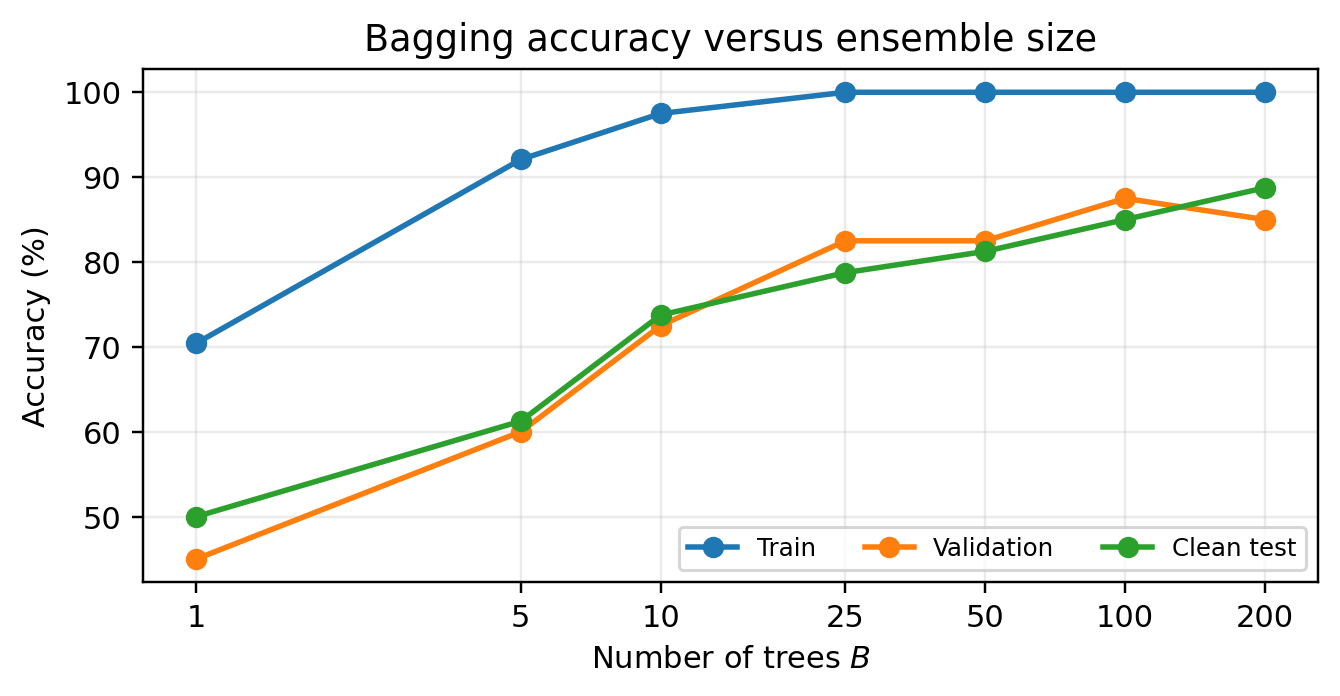
\includegraphics[width=\columnwidth]{figures/q1_bagging_accuracy.png}
\caption{Train, validation, and clean-test accuracy as the number of bagged trees increases. Selection uses validation accuracy.}
\label{fig:bagacc}
\end{figure}

\begin{table}[t]
\centering
\caption{Q1(c): OOB diagnostics. Disagreement is undefined for one tree.}
\label{tab:oob}
\scriptsize
\begin{tabular}{r|rrr}
\toprule
$B$ & OOB acc. & Disagr. & Margin\\
\midrule
1 & 0.3780 & -- & 1.0000\\
5 & 0.3412 & 0.7838 & 0.2475\\
10 & 0.4059 & 0.7831 & 0.2650\\
25 & 0.5792 & 0.7902 & 0.2625\\
50 & 0.6542 & 0.7883 & 0.2718\\
100 & 0.7125 & 0.7891 & 0.2768\\
200 & 0.7333 & 0.7962 & 0.2739\\
\bottomrule
\end{tabular}
\end{table}

\begin{figure}[t]
\centering
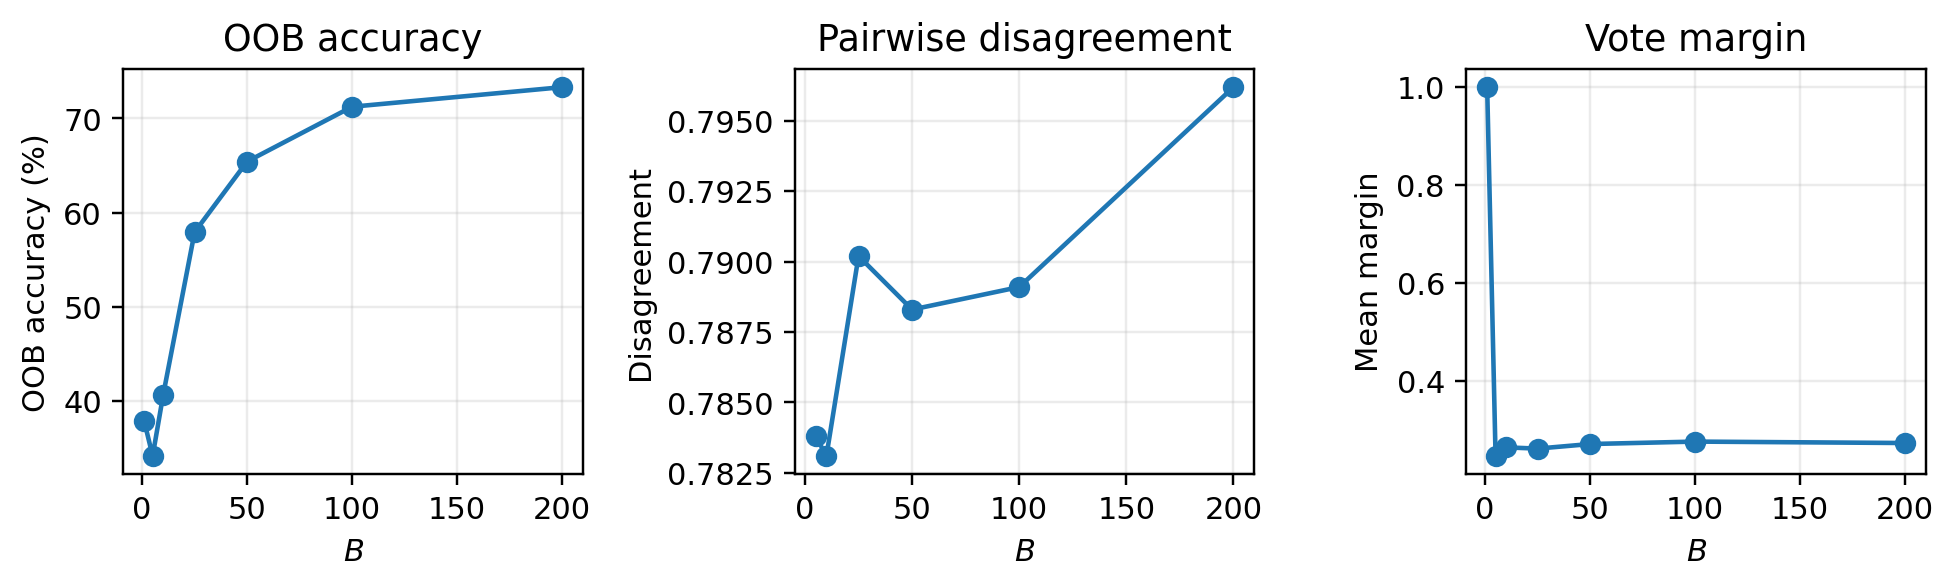
\includegraphics[width=\columnwidth]{figures/q1_oob_disagreement_margin.png}
\caption{OOB accuracy, average pairwise disagreement, and mean vote margin versus ensemble size.}
\label{fig:oob}
\end{figure}

\subsection{Clean and masked test comparison}
The frozen tree remains at 50.0\% on clean and masked test images, with mean leaf probability 0.9765. Bagging falls from 85.0\% to 73.75\%; its mean winning vote fraction falls from 0.3790 to 0.2692. In two inspected masked examples, bagging corrects the tree (original image indices 4 and 27); in two other cases both models are wrong (indices 1 and 21). The vote distributions show that aggregation can correct sample-specific tree errors when voters differ, but cannot guarantee a correction when the available pixels support a shared wrong identity.

\begin{table}[t]
\centering
\caption{Q1(d): selected test-face examples. Vote entries show the leading bagging classes and counts.}
\label{tab:q1faces}
\scriptsize
\begin{tabular}{r|r|r|r|r|l}
\toprule
Image & True & Tree & Bag & Case & Leading votes\\
\midrule
4 & 0 & 29 & 0 & Corrected & $0$:21, $1$:14\\
27 & 2 & 4 & 2 & Corrected & $2$:19, $30$:12\\
1 & 0 & 29 & 25 & Both wrong & $25$:9, $30$:8, $33$:8\\
21 & 2 & 29 & 33 & Both wrong & $33$:16, $30$:11, $3$:9\\
\bottomrule
\end{tabular}
\end{table}

\section{Q2: Multiclass SAMME Boosting}
\subsection{One-round verification and model selection}
The nine-sample, three-class toy example starts with weight $1/9$ per sample. A depth-1 stump makes three errors, giving $\epsilon=1/3$, below the random threshold $2/3$. Its SAMME coefficient is 1.3863; after normalization, correctly classified points have weight 0.05556 and misclassified points 0.22222. The updated weights sum to one.

For the face data, depths $\{1,2,3,4\}$ and rounds $\{10,25,50,100\}$ are evaluated on clean validation images. The selected model is depth 4 with 100 rounds and validation accuracy 41.25\%. All 100 weak learners are accepted under the 40-class threshold 0.975. Figure~\ref{fig:samme} shows validation accuracy and the selected model's round dynamics.

\begin{figure}[t]
\centering
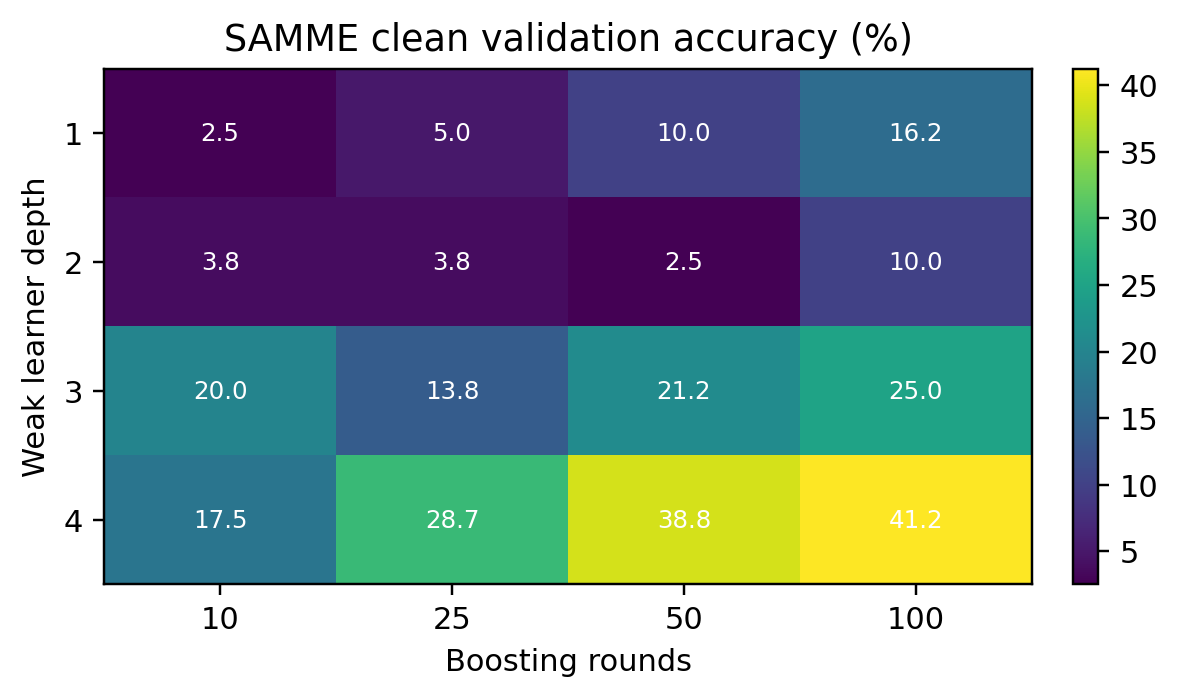
\includegraphics[width=\columnwidth]{figures/q2_samme_validation_grid.png}
\caption{Clean validation accuracy for the 16 depth--round SAMME configurations.}
\label{fig:samme}
\end{figure}
\begin{figure}[t]
\centering
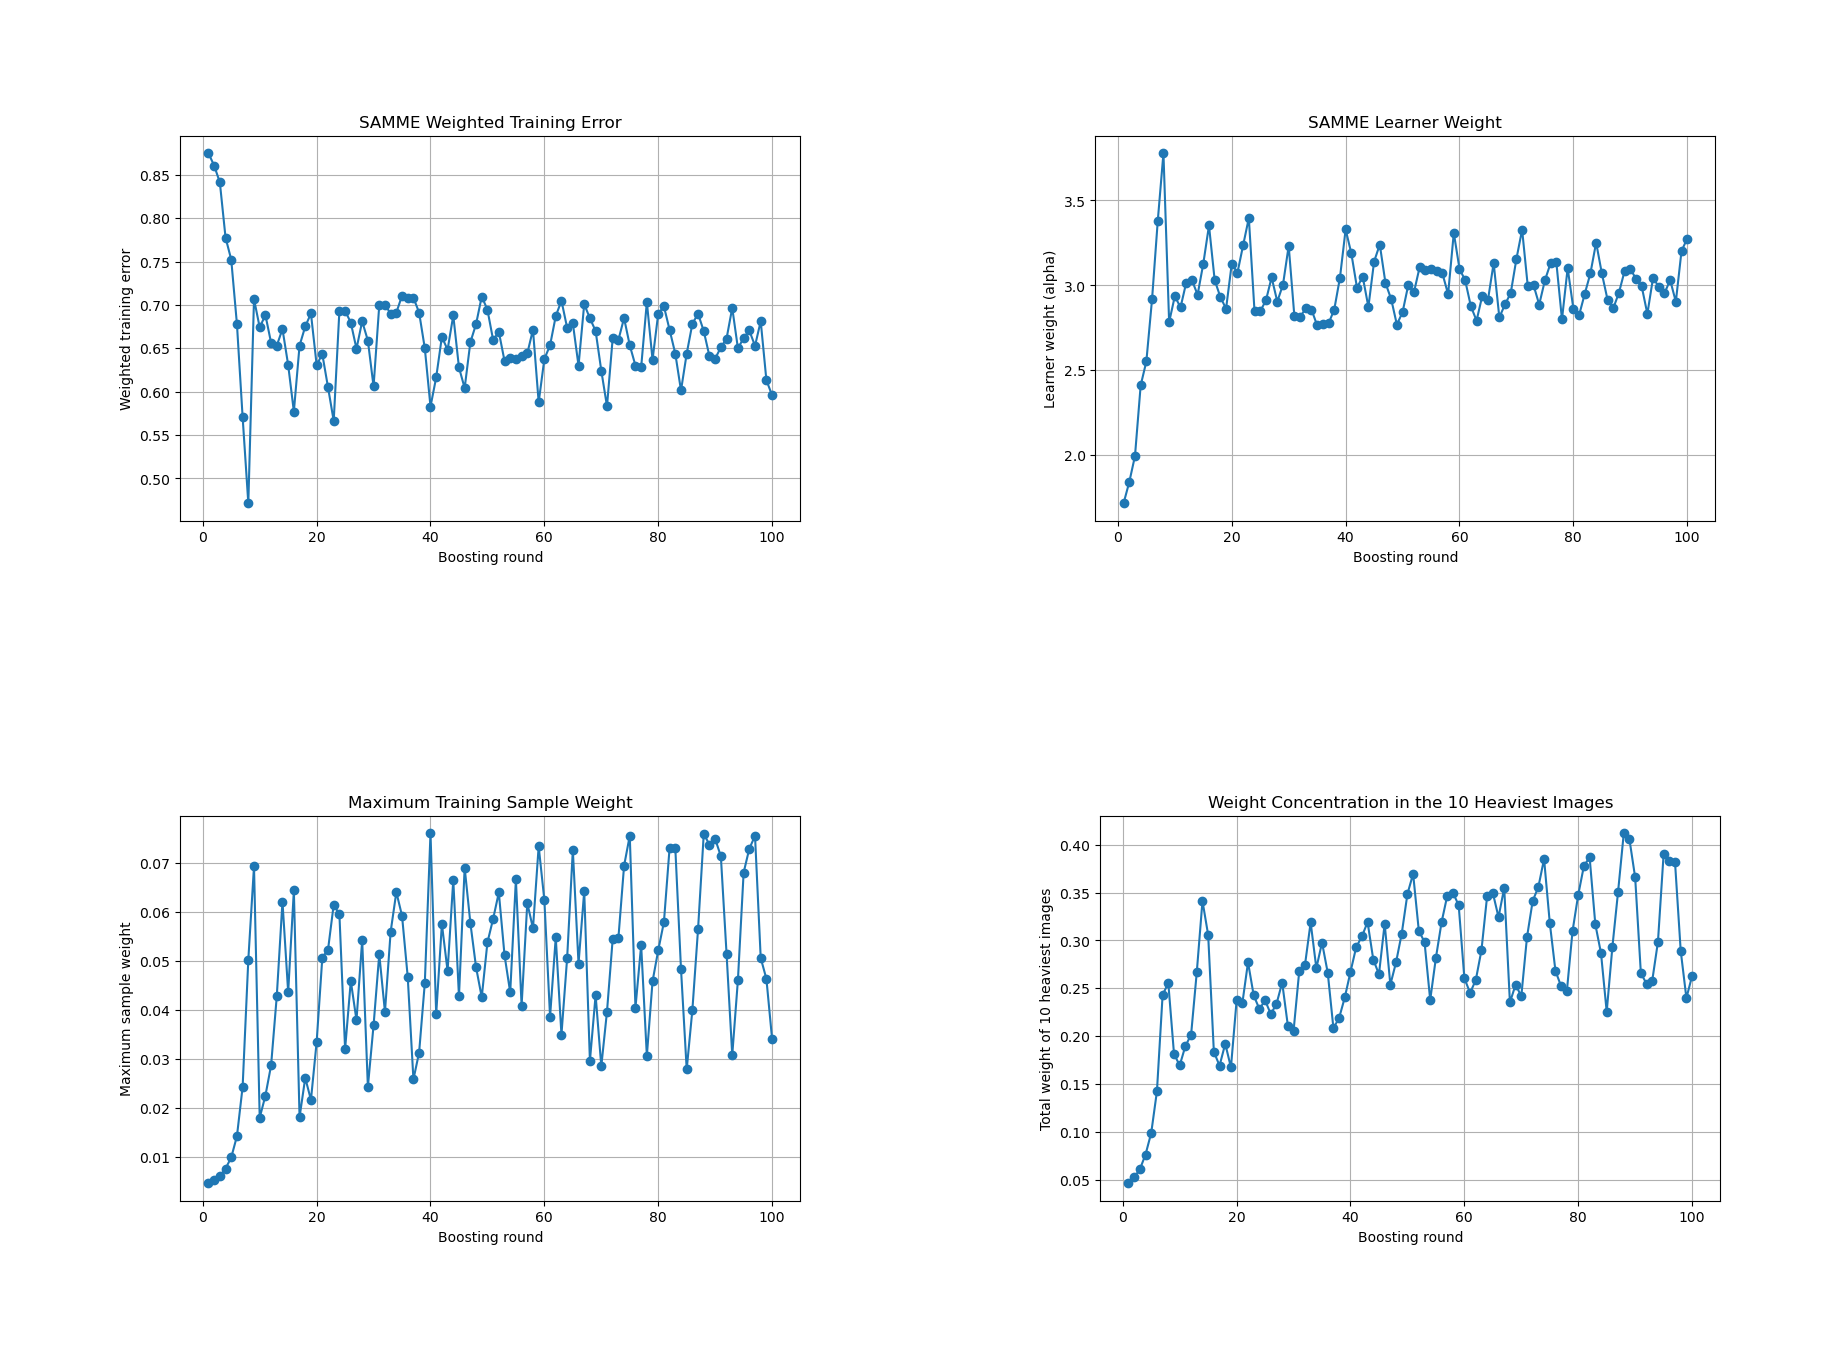
\includegraphics[width=\columnwidth]{figures/q2_samme_training_dynamics.png}
\caption{Selected SAMME model: weighted training error, $\alpha_t$, maximum sample weight, and weight mass on the ten heaviest samples.}
\label{fig:boostdyn}
\end{figure}

\begin{figure}[t]
\centering
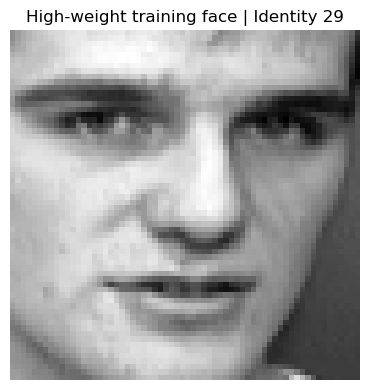
\includegraphics[width=0.58\columnwidth]{figures/q2_high_weight_face.png}
\caption{Training image (identity 29) attaining the largest recorded SAMME sample weight.}
\label{fig:hardface}
\end{figure}

\subsection{Bagging versus boosting and a difficult face}
At 100 learners, bagging reaches 100.0\% train, 87.5\% validation, and 85.0\% test accuracy in 64.76 s of cumulative tree fitting. SAMME reaches 98.75\%, 41.25\%, and 40.0\% in 19.81 s. The 25- and 50-learner comparisons are reported in the repository logs. These times measure weak-learner fitting only, excluding prediction and bootstrap overhead. One training face (dataset index 292, identity 29) reaches weight 0.07616 at round 40. Its round-wise predictions repeatedly miss the true identity, causing the SAMME update to increase its weight after errors and decrease it after a correct prediction. This is the intended re-focusing mechanism, although it does not guarantee that later weak learners can represent that face well.

\begin{table}[t]
\centering
\caption{Q2(c): bagging and SAMME comparison. Fit time sums calls to each learner's \texttt{fit} method.}
\label{tab:q2compare}
\scriptsize
\begin{tabular}{r|l|rrr|r}
\toprule
Learners & Model & Train & Val. & Test & Time (s)\\
\midrule
25 & Bagging & 100.00 & 82.50 & 78.75 & 16.41\\
25 & SAMME & 80.00 & 28.75 & 28.75 & 4.83\\
50 & Bagging & 100.00 & 82.50 & 81.25 & 32.79\\
50 & SAMME & 90.00 & 38.75 & 23.75 & 9.73\\
100 & Bagging & 100.00 & 87.50 & 85.00 & 64.76\\
100 & SAMME & 98.75 & 41.25 & 40.00 & 19.81\\
\bottomrule
\end{tabular}
\end{table}

\subsection{Clean and masked test comparison}
The selected SAMME model changes from 40.0\% clean to 45.0\% masked test accuracy, with mean winning weighted vote 0.1205 and 0.1163, respectively. On one inspected test face, bagging predicts identity 4 both before and after masking, while SAMME changes from identity 4 to 12. For that face, bagging pairwise disagreement rises from 0.7418 to 0.9057 and 65\% of trees flip their individual prediction, even though the aggregate bagging label stays fixed. The fraction of total SAMME learner weight attached to weak learners that flip is 0.0609. The boosted vote therefore changes because its alpha-weighted voters are not the same as the unweighted bagging majority.

\begin{table}[t]
\centering
\caption{Q2(d): clean/masked accuracy and mean winning confidence.}
\label{tab:q2robust}
\scriptsize
\begin{tabular}{l|rrrr}
\toprule
Model & Clean acc. & Masked acc. & Clean conf. & Masked conf.\\
\midrule
Single tree & 50.00 & 50.00 & 0.9765 & 0.9765\\
Bagging & \textbf{85.00} & 73.75 & 0.3790 & 0.2692\\
SAMME & 40.00 & 45.00 & 0.1205 & 0.1163\\
\bottomrule
\end{tabular}
\end{table}

\begin{figure}[t]
\centering
\begin{minipage}{0.48\columnwidth}
\centering
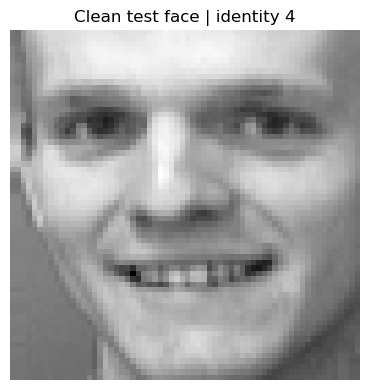
\includegraphics[width=\linewidth]{figures/q2d_clean_face.png}
\end{minipage}\hfill
\begin{minipage}{0.48\columnwidth}
\centering
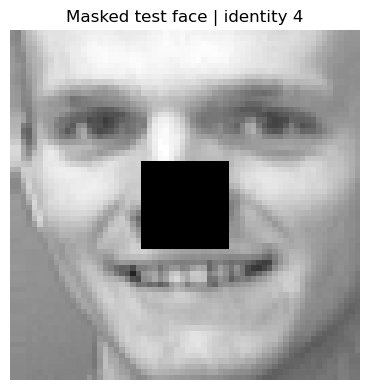
\includegraphics[width=\linewidth]{figures/q2d_masked_face.png}
\end{minipage}
\caption{Inspected identity-4 test face before and after central masking.}
\label{fig:maskface}
\end{figure}

\section{Q3: Measured Bias and Variance}
\subsection{Thirty-refit measurement}
Across 30 within-identity resamples, the single tree has bias squared 0.4090 and variance 0.6566; bagging has 0.5322 and 0.0245; SAMME has 0.8801 and 0.0180. Mean test accuracy and sample standard deviation are 46.71\% (0.0495), 76.79\% (0.0385), and 29.08\% (0.0754), respectively. Bagging provides the strongest average accuracy and the smallest run-to-run accuracy standard deviation. SAMME has the lowest probability-vector variance but substantially larger bias squared and poorer accuracy.

\begin{table}[t]
\centering
\caption{Q3(a): measured bias, variance, and accuracy over 30 refits.}
\label{tab:q3a}
\small
\begin{tabular}{l|rrrr}
\toprule
Model & Bias$^2$ & Var. & Mean acc. & Std.\\
\midrule
Tree & 0.4090 & 0.6566 & 46.71 & 0.0495\\
Bagging & 0.5322 & 0.0245 & \textbf{76.79} & \textbf{0.0385}\\
SAMME & 0.8801 & \textbf{0.0180} & 29.08 & 0.0754\\
\bottomrule
\end{tabular}
\end{table}

\subsection{Depth dependence and variance removed by bagging}
The original Q1(a) setting is unrestricted depth (\texttt{None}); its fitted tree realizes depth 34. Since an unrestricted parameter has no larger numeric cap, Q3(b) uses this realized depth as the finite selected-depth reference, then compares caps 2, 34, and 68. This interpretation is explicit but is a proxy for refitting the original \texttt{None} parameter. At depth 34, bagging improves mean accuracy by 28.71 percentage points; at depth 68 it improves by 27.33 points. Although depth 68 removes slightly more variance (0.6129 versus 0.5717), it does not yield the largest accuracy gain.

\begin{table}[t]
\centering
\caption{Q3(b): depth-wise measured errors, mean accuracy, sample standard deviation, and bagging accuracy improvement (percentage points).}
\label{tab:q3b}
\scriptsize
\begin{tabular}{r|l|rrrrr}
\toprule
Depth & Model & Bias$^2$ & Var. & Acc. & Std. & $\Delta$Acc.\\
\midrule
2 & Tree & 0.9092 & 0.0466 & 6.29 & 0.0116 & --\\
2 & Bagged & 0.9296 & 0.0105 & 15.46 & 0.0661 & +9.17\\
34 & Tree & 0.3886 & 0.5964 & 48.12 & 0.0539 & --\\
34 & Bagged & 0.5330 & 0.0247 & 76.83 & 0.0436 & +28.71\\
68 & Tree & 0.3750 & 0.6376 & 49.38 & 0.0542 & --\\
68 & Bagged & 0.5323 & 0.0247 & 76.71 & 0.0424 & +27.33\\
\bottomrule
\end{tabular}
\end{table}

\begin{figure}[t]
\centering
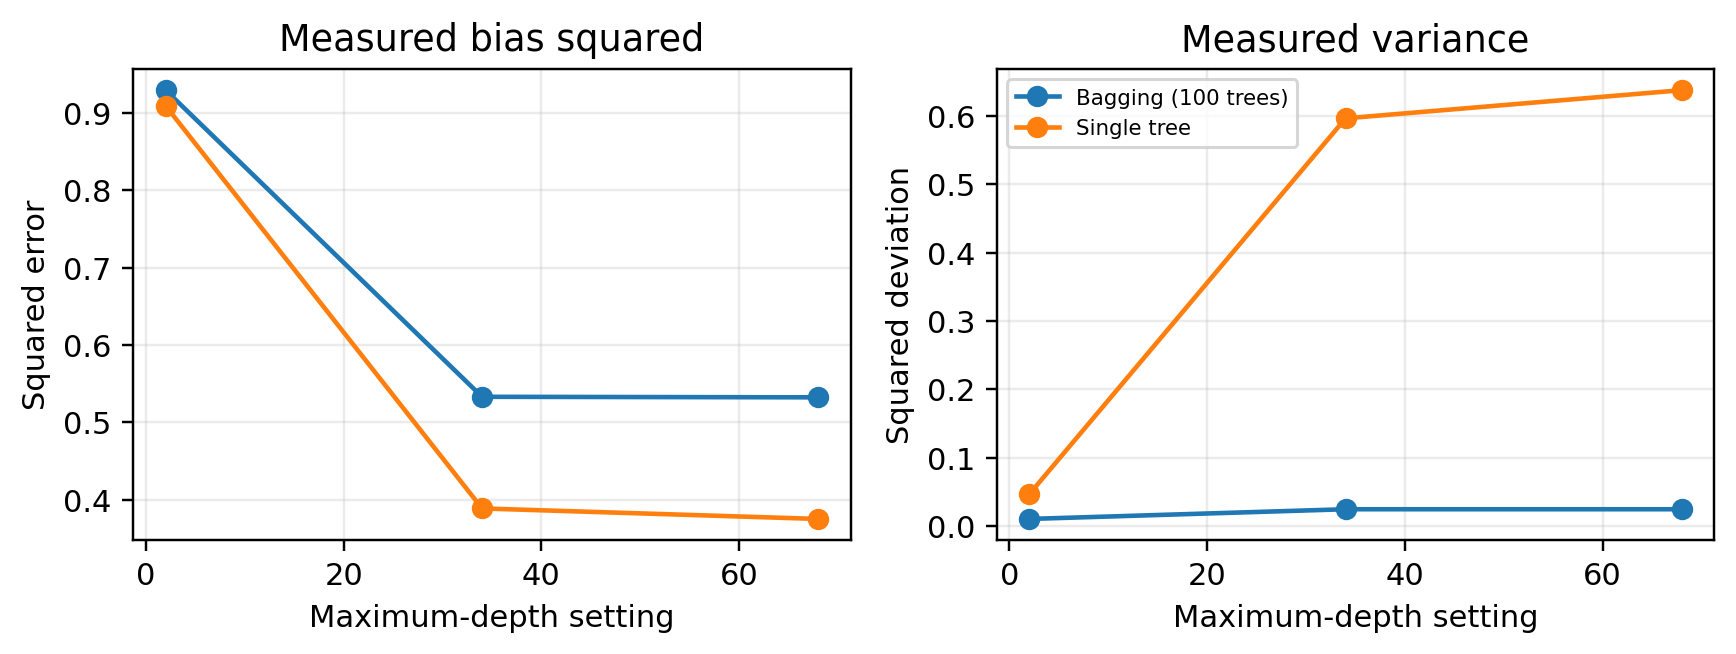
\includegraphics[width=\columnwidth]{figures/q3_depth_bias_variance.png}
\caption{Measured bias squared and variance for single trees and 100-tree bagging across depth settings.}
\label{fig:q3depth}
\end{figure}

\subsection{Leaf occupancy and disagreement}
First-repetition structural diagnostics show leaf counts of 3, 36, and 40 for single trees at depths 2, 34, and 68. Mean samples per leaf decrease from 80.0 to 6.67 and 6.0. The corresponding mean bagged-tree leaf counts are 3.17, 39.11, and 39.23. Pairwise disagreement on the fixed clean test set is 0.9636, 0.8314, and 0.8310. Thus, the largest depth has the greatest measured variance reduction, but its disagreement is essentially the same as the selected-depth case and its accuracy improvement is smaller. These diagnostics were computed for the first of the 30 resampling repetitions, not averaged across repetitions.

\begin{table}[t]
\centering
\caption{Q3(c): first-repetition structural diagnostics (not 30-repetition averages).}
\label{tab:q3diag}
\scriptsize
\begin{tabular}{r|rr|rr|r}
\toprule
Depth & Single leaves & Single $n$/leaf & Bag leaves & Bag $n$/leaf & Disagr.\\
\midrule
2 & 3 & 80.00 & 3.17 & 76.60 & 0.9636\\
34 & 36 & 6.67 & 39.11 & 6.14 & 0.8314\\
68 & 40 & 6.00 & 39.23 & 6.12 & 0.8310\\
\bottomrule
\end{tabular}
\end{table}

\subsection{Final model comparison}
Table~\ref{tab:final} combines clean and masked test accuracy with Q3(a) bias squared and variance. Bagging is the most accurate on clean and masked test images and has the lowest standard deviation of accuracy across refits. SAMME has the lowest prediction-vector variance but the largest bias squared and worst clean accuracy. Bagging is most affected by the central mask in aggregate accuracy (an 11.25-point decrease); the single-tree score is unchanged and SAMME rises by five points on this particular fixed test set. Therefore, lowest measured variance is not equivalent to best test accuracy, and the observed masking effect is dataset- and model-dependent.

\begin{table}[t]
\centering
\caption{Q3(d): final selected-model comparison.}
\label{tab:final}
\small
\begin{tabular}{l|rrrr}
\toprule
Model & Clean & Masked & Bias$^2$ & Var.\\
\midrule
Single tree & 50.00 & 50.00 & 0.4090 & 0.6566\\
Bagging & \textbf{85.00} & \textbf{73.75} & 0.5322 & 0.0245\\
SAMME & 40.00 & 45.00 & 0.8801 & \textbf{0.0180}\\
\bottomrule
\end{tabular}
\end{table}

\begin{figure}[t]
\centering
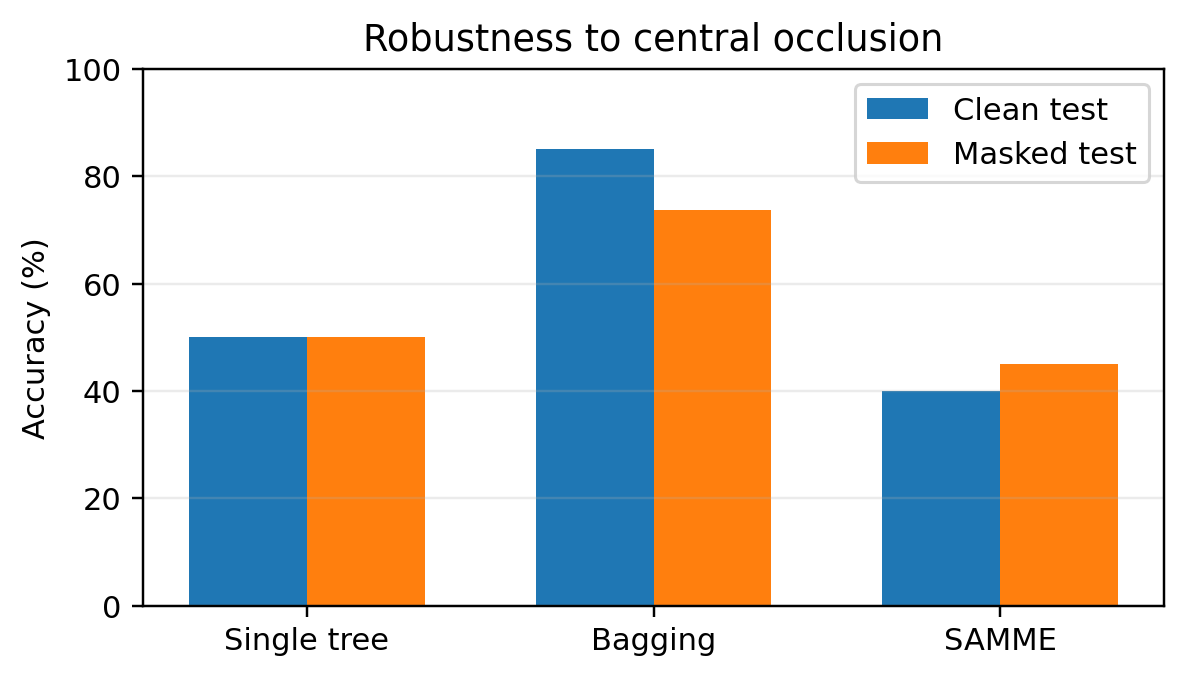
\includegraphics[width=\columnwidth]{figures/q3_final_clean_masked_accuracy.png}
\caption{Final clean and masked test accuracy for the selected models.}
\label{fig:robust}
\end{figure}

\section{Conclusion and Reproducibility Notes}
On this fixed split, bagging is the strongest classifier by clean test accuracy and is the most stable when stability is measured as the standard deviation of accuracy over 30 refits. SAMME has the smallest prediction-vector variance, but that concentration around incorrect predictions accompanies high bias and lower accuracy. Increasing tree depth does not make bagging's accuracy gain increase monotonically: the selected-depth case improves more than the deeper case, despite the latter's slightly greater variance reduction. The saved split, executed notebook, configurations, CSV/JSON logs, figure-generation script, environment files, and exact commands are packaged with the submission. The GitHub URL and commit hash on page one identify the submitted repository revision provided for this report.

\clearpage
\begin{thebibliography}{9}
\bibitem{breiman96}
L. Breiman. Bagging predictors. \emph{Machine Learning}, 24:123--140, 1996.

\bibitem{zhu09}
J. Zhu, H. Zou, S. Rosset, and T. Hastie. Multi-class AdaBoost. \emph{Statistics and Its Interface}, 2(3):349--360, 2009.

\bibitem{pedregosa11}
F. Pedregosa et al. Scikit-learn: Machine learning in Python. \emph{Journal of Machine Learning Research}, 12:2825--2830, 2011.

\bibitem{sklearnfaces}
Scikit-learn developers. The Olivetti faces dataset. \emph{Scikit-learn API documentation}. \url{https://scikit-learn.org/stable/modules/generated/sklearn.datasets.fetch_olivetti_faces.html}.

\bibitem{cvprkit}
CVPR Organizing Committee. CVPR author kit, official two-column LaTeX author resources. \url{https://github.com/cvpr-org/author-kit}.
\end{thebibliography}
\end{document}
